\newpage
\section{The Physical Layer}
最底层, network基础. 最小单位: bit. 不同 physical channels 决定 throughput, latency (delay) and error rate. 

\subsection{The theoretical basis for data communication}
\subsubsection{Fourier Series}
信息通过改变物理量来传输. 

Any reasonably behaved \textbf{periodic} function $g(t)=g(t+nT_0)$ with period $T$ can be represented as
\begin{align*}
    g(t)&=\sum_{n=-\infty}^{+\infty}a_n e^{j\textcolor{light_red}{2\pi fn}t}\\
    &=\sum_{n=-\infty}^{+\infty} a_n (\cos(\textcolor{light_red}{2\pi fn}t)+j\sin(\textcolor{light_red}{2\pi fn}t))
\end{align*}
where $f_0=\frac{1}{T_0}$ is \textbf{the fundamental frequency} of the periodic signal $g(t)$. 

If the period $T_0$ is known and the amplitudes an are given, the original periodic signal $g(t)$ can be reconstructed. 也可反求 $a_n$. 
\begin{align*}
    a_n=\frac{1}{T}\int_T g(t)e^{-j\textcolor{light_red}{2\pi fn}t}dt
\end{align*}


If $g(t)$ is a \textbf{real} signal, then the coefficient $a_{-n}$ is \textbf{the conjugate} of $a_n$.
\begin{align}
    g(t)&=C+\sum_{n=1}^{\infty}2A_n\cos (2\pi nft)+\sum_{n=1}^\infty 2B_n\sin (2\pi n ft)\\
    \notag A_n&=\frac{1}{T}\int_0^T g(t)\cos(2\pi nft)dt\\
    \notag B_n&=\frac{1}{T}\int_0^T g(t)\sin(2\pi nft)dt\\
    \notag C  &=\frac{1}{T}\int_0^T g(t)dt
\end{align}

但现实世界信号有限, 但可以假想为重复的无限信号, 如此可用 Fourier. 
%TODO P8 算一算

\subsubsection{Bandwidth-limited Signals}
信号在信道传输会衰减. 且信道对不同频率的影响不同. 但对某一根线, 振幅从0到$f_c$(the cutoff frequency, 截止频率)之前信号衰减很小. 

The width of the frequency range transmitted without being strongly attenuated is called the \textbf{bandwidth}(带宽). (带宽是没有大量衰减的范围) 带宽是物理属性, 不依赖于环境. 

\paragraph{Baseband Signals vs. Passband Signals}\quad
\begin{itemize}
    \item Signals that run from 0 up to a maximum frequency are called basedband signals.
    \item Signals are shifted to occupy a higher range of frequencies, such as in the case of all wireless transmission, are called passband signals.
\end{itemize}

$f_c$ carrier frequency

\paragraph{Bandwidth vs. Maximum Data Rate}
\begin{itemize}
    \item analogue bandwidth is a quantity measured in Hz.
    \item digital bandwidth is the maximum data rate of a channel, a quantity measured in bits/sec.
\end{itemize}
data rate 是使用 analogue bandwidth 最终传输结果. 


\subsubsection{The Maximum Data Rate of a Channel}
Channel Capacity --- the maximum rate at which data can be transmitted over a given communication path or channel under given conditions.

Four related concepts:
\begin{enumerate}
    \item Data rate (bps)
    \item Bandwidth (Hz)
    \item Noise
    \item Error rate
\end{enumerate}

\subsubsection{Nyquist Bandwidth}
在理想情况下的 the maximum signaling rate
\begin{align*}
    s(t)=\sum_n a_n g(t-nT)
\end{align*}
where $g(t)$ represents a basic pulse shape and $\{a_n\}$ is the binary sequence of $\{\pm 1\}$ transmitted at a rate of $\frac{1}{T}$ bits/s.

The optimal pulse shape: %(C 是 capacity, B 是 bandwidth) 
\begin{align*}
    g(t)=\frac{\sin 2\pi Bt}{2\pi Bt}
\end{align*}
\begin{itemize}
    \item Binary: \textcolor{light_red}{$C = 2B$} (V=2)
    \item Multilevel Signaling: \textcolor{light_red}{$C = 2B \log_2 V$} ($V$ is the number of discrete signal or voltage levels)
\end{itemize}
提升信号种类的数量可以提升data rate. 但提升有限度, 且会被在传输中的 noise and other impairment 限制. 

\subsubsection{Shannon Capacity}
仅假设白噪声, 不考虑其他影响, 仅理论最大值. SNR (信噪比)
\begin{align*}
    C&=B\log_2 (1+SNR)\\
    SNR_{dB}&=10\lg\frac{\text{signal power}}{\text{noise power}}=10\lg(SNR)
\end{align*}

\subsection{Three kinds of transmission media}
\subsubsection{Guided Transmission Media}
\begin{itemize}
    \item Persistent storage (固态存储)
    \item Twisted pairs (双绞线)
    \item Coaxial cable (同轴线缆)
    \item Power lines (交流电的线)
    \item Fiber optics (光纤)
\end{itemize}

\paragraph{Persistent storage} 卡车运硬盘仍是最高的 bandwidth. 但 delay 很大. 

\paragraph{Twisted pairs} 最古老但仍最常用的传输介质. 为什么要绞: 因为两根平行线会形成一个小天线, 纠缠会抵消其干扰. 一个信号是这两根线的电压差, 提升鲁棒性. 

\begin{figure}[!htb]
    \centering
    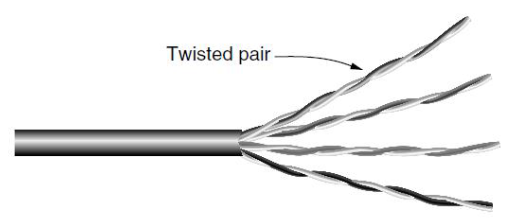
\includegraphics[width=0.309\textwidth]{pic/CN2/Twisted pairs.png}
    \caption{Twisted pairs}
\end{figure}

\paragraph{Coaxial Cable}黄铜轴x
\begin{figure}[!htb]
    \centering
    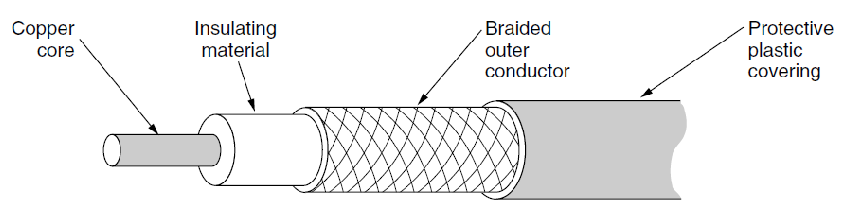
\includegraphics[width=0.42\textwidth]{pic/CN2/Coaxial Cable}
    \caption{Coaxial Cable}
\end{figure}

\paragraph{Power Lines}交流电的线. 中国民用交流电: 50Hz
\begin{figure}[!htb]
    \centering
    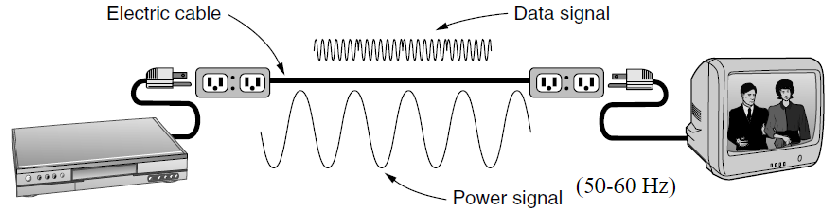
\includegraphics[width=0.42\textwidth]{pic/CN2/Power Lines}
    \caption{Power Lines}
\end{figure}

\paragraph{Fiber Optics}理论上 bandwidth可以无限大. 

重要组成部分: Light source, transmission medium, and detector. 

光源: LEDs, Semiconductor lasers.

\begin{figure}[!htb]
    \centering
    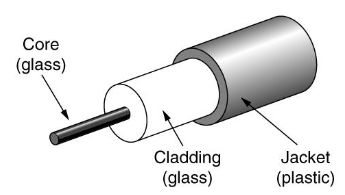
\includegraphics[width=0.309\textwidth]{pic/CN2/Fiber Optics}
    \caption{Fiber Optics}
\end{figure}

\subsubsection{Wireless}
three variations:
\begin{itemize}
    \item Frequency hopping spread spectrum
    \item Direct sequence spread spectrum e.g. CDMA
    \item UWB (Ultra WideBand)
\end{itemize}

\paragraph{Radio Transmission} Radio frequency (RF) waves 

\paragraph{Microwave Transmission} 传输是直线. 

\subsection{Digital modulation and multiplexing}
\subsection{Three examples of communication examples}